
\section{DDPG}\label{DDPGsection}

\subsection{Вывод из Deep Q-learning}

Схема DQN \ref{DQNalgorithm} имела принципиальный недостаток: мы не могли работать с непрерывными пространствами действий в силу необходимости постоянно считать операторы максимума и аргмаксимума
$$\max_a Q^*(s, a, \theta)$$
как для жадного выбора действия, так и для построения таргета в задаче регрессии. 

\needspace{7\baselineskip}
\begin{wrapfigure}{r}{0.35\textwidth}
\vspace{-0.3cm}
\centering
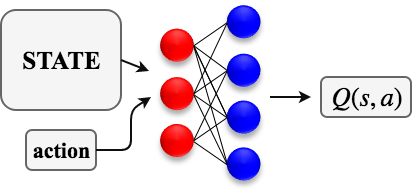
\includegraphics[width=0.3\textwidth]{Images/Qnetwork1.png}
\vspace{-0.3cm}
\end{wrapfigure}

Единственная возможная архитектура модели --- приём действий на вход вместе с состояниями, тогда поиск аргмаксимума проводить, в целом, можно, но дорого: инициализируем $a^0$ случайно, и устраиваем градиентный подъём по входу в модель:
$$a^{k+1} = a^k + \alpha \left. \nabla_a Q^*(s, a, \theta) \right|_{a = a^k}$$

Понятно, что такую процедуру устраивать по несколько раз за шаг дороговато. Однако, в глубинном обучении для таких проблем есть мега-универсальное решение: давайте задачу поиска аргмаксимума тоже аппроксимируем другой нейросетью! Максимум тогда можно будет считать, просто подставив в $Q^*$ вместо действия приближение этого аргмаксимума.

Итак, пусть $\pi(s, \omega)$ принимает на вход состояние $s$ и выдаёт аргмаксимум текущей аппроксимации Q-функции, то есть будем добиваться $\pi(s, \omega) = \argmax\limits_a Q^*(s, a, \theta)$. Понятно, как обучать такую сеть:
$$Q^*(s, \pi(s, \omega), \theta) \to \max_{\omega}$$

Весь алгоритм DQN оставляем неизменным с единственной модификацией, что на каждом батче также нужно сделать шаг оптимизации $\omega$. При этом каждый раз, когда в схеме необходимо считать максимум или аргмаксимум $Q^*$, используется $\pi(s, \omega)$.

Посмотрим, что нам нужно копировать для таргет-сети. В стандартном алгоритме DQN нам было необходимо считать $\max\limits_{a'} Q^*(s', a', \theta^{-})$. Значит, для таргет-сети $Q^*(s', a', \theta^{-})$ нам тоже нужно знать аргмаксимум, для чего будем хранить старую версию вспомогательной функции $\pi(s, \omega^{-})$.

Итого мы получили, что для жадного выбора действия используется $\pi(s, \omega)$ (отсюда такое обозначение этой <<вспомогательной>> функции); а таргет для перехода $\T \coloneqq (s, a, r, s')$ вычисляется по формуле
$$y(\T) \coloneqq r + \gamma Q^*(s', \argmax_{a'} Q^*(s', a', \theta^{-}), \theta^{-}) \approx r + \gamma Q^*(s', \pi(s, \omega^{-}), \theta^{-})$$

\begin{remark}
Все модификации DQN (за исключением дуэльной архитектуры) $Q$-сетки переносимы на случай DDPG. Чтобы воспользоваться идеей Double DQN, таргет-сеть нужна только для оценки выбранного текущей версией действия $a'$, поэтому при использовании этой идеи достаточно хранить только $Q^*(s', a', \theta^{-})$.
\end{remark}

\subsection{Вывод из Policy Gradient}

% В Policy Gradient подходе мы могли работать с непрерывными пространствами действий, например, выдавая стратегией $\pi$ среднее и диагональную матрицу ковариации из нормального распределения:
% $$\pi_\theta(a \mid s) = \N\left( \mu(s, \theta), \sigma^2(s, \theta)I \right)$$

В Policy Gradient алгоритмах мы получили формулу градиента нашего функционала, <<релаксировав>> задачу и перейдя к оптимизации в пространстве стохастических стратегий. Если пространство действий непрерывно, то такая релаксация на самом деле не обязательна. Предположим\footnote{даже если это не так, в будущем мы всё равно будем приближать эти Q-функции нейросетями, для которых всегда справедлива дифференцируемость по входу.} дифференцируемость любых Q-функций $Q^{\pi}(s, a)$ по действиям $a$. Попробуем посчитать градиент по параметрам стратегии в случае детерминированной стратегии $a = \pi_\theta(s)$:

\begin{theorem}
\begin{equation}\label{dpg}
\nabla_\theta J(\pi_\theta) = \frac{1}{1 - \gamma}\E_{d_{\pi_\theta}(s)} \nabla_\theta \pi_\theta(s) \left. \nabla_a Q^{\pi}(s, a) \right|_{a = \pi_\theta(s)}
\end{equation}
\beginproof
$$\nabla_\theta V^{\pi}(s) = \{\text{VQ уравнение \eqref{VQ}}\} = \nabla_\theta \E_{a \sim \pi_\theta(s)} Q^{\pi}(s, a) = \nabla_\theta Q^{\pi}(s, \pi_\theta(s)) = (*)$$
Заметим, что в последнем выражении при малом изменении $\theta$ поменяется не только $\pi_\theta(s)$, но и сама оценочная функция $Q^\pi$. Считая, что якобиан функции $\R^n \to \R^m$ имеет размерность $n \times m$, размерности градиентов будут следующие:
$$\nabla_\theta Q^{\pi}(s, a) \in \R^{\Theta \times 1} \quad \nabla_a Q^{\pi}(s, a) \in \R^{\A \times 1} \quad \nabla_\theta \pi_\theta(s) \in \R^{\Theta \times \A}$$
Тогда продолжение вычисления выглядит так:
$$(*) = \nabla_\theta \pi_\theta(s) \left. \nabla_a Q^{\pi}(s, a) \right|_{a = \pi_\theta(s)} + \left. \nabla_\theta Q^{\pi}(s, a) \right|_{a = \pi_\theta(s)}$$
где последнее слагаемое --- якобиан $Q^{\pi}$ при фиксированном $a$ по стратегии $\pi$, которую он оценивает. Отдельно это слагаемое имеет вид:
$$\nabla_\theta Q^{\pi}(s, a) = \{\text{QV уравнение \eqref{QV}} \} = \gamma \E_{s'} \nabla_\theta V^{\pi}(s')$$

Получаем рекурсивную формулу, аккуратно собирая которую, получим:
$$\nabla_\theta V^{\pi}(s) = \E_{\Traj \sim \pi \mid s_0 = s} \sum_{t = 0} \gamma^t \nabla_\theta \pi_\theta(s_t) \left. \nabla_a Q^{\pi}(s_t, a) \right|_{a = \pi_\theta(s_t)}$$

Осталось только применить теорему \eqref{th:decoupling_stoch} об эквивалентной форме мат.ожидания по траекториям для 
\begin{equation*}
f(s, a) = \nabla_\theta \pi_\theta(s) \left. \nabla_a Q^{\pi}(s, a) \right|_{a = \pi_\theta(s)}   \tagqed
\end{equation*}
\end{theorem}

Сразу построим суррогатную функцию для такой формулы градиента:
$$\mathcal{L}_{\textcolor{ChadPurple}{\tilde{\pi}}}(\textcolor{ChadBlue}{\theta}) \coloneqq \frac{1}{1 - \gamma}\E_{\textcolor{ChadPurple}{d_{\tilde{\pi}}(s)}} Q^{\textcolor{ChadPurple}{\tilde{\pi}}}(s, \textcolor{ChadBlue}{\pi_{\theta}}(s))$$
Действительно, если мы посчитаем градиент этой функции по $\theta$, то мы просто получим формулу chain rule для оптимизации параметров стратегии через градиент Q-функции по действиям. Иными словами, градиент по параметрам детерминированной стратегии указывает просто проводить policy improvement: выбирать те действия, для которых Q-функция больше, используя её градиент по действиям.

Если мы хотим построить Actor-Critic схему, воспользовавшись такой формулой, нам придётся аппроксимировать Q-функцию и явно использовать её градиент по действиям. Таким образом, обойтись обучением лишь V-функции или пользоваться многошаговыми оценками не получится, поэтому преимуществами on-policy подхода в такой формуле воспользоваться не удастся.

Можем ли мы воспользоваться формулой в off-policy режиме? Вообще говоря, нет, поскольку состояния должны приходить согласно формуле из распределения $d_{\pi_\theta}(s)$. Однако, вспоминая концепцию policy improvement-а (теорема \ref{th:policyimprovement}), мы понимаем, что если мы будем оптимизировать Q-функцию по действиям, то как бы мы это не делали (из какого бы распределения не брали состояния, в которых мы изменяем стратегию), мы всё равно сможем увеличить значение нашего функционала. Это означает, что если мы в формуле \eqref{dpg} заменим $d_{\pi_\theta}(s)$ на что-либо другое, полученная формула <<градиента>> будет всё равно направлением улучшения стратегии, пусть и не направлением локально максимального увеличения функционала, что верно для честного градиента. Итого, будем сэмплировать батч состояний из реплей буфера и делать шаг градиентного подъёма: 
$$\theta \leftarrow \theta + \alpha \E_{s} \nabla_\theta \pi_\theta(s) \left. \nabla_a Q^{\pi}(s, a) \right|_{a = \pi_\theta(s)},$$
что эквивалентно одному шагу градиентной оптимизации суррогатной функции:
\begin{equation}\label{ddpg_actor}
\E_s Q^{\pi}(s, \pi_{\theta}(s)) \to \max_{\theta}
\end{equation}

Q-функцию, необходимую для такой оптимизации, будем тоже учить в off-policy режиме с одношаговых оценок: тогда ему для данной пары $s,a$ требуется лишь сэмпл $s'$, поэтому такого критика можно обучать по переходам $\T \coloneqq (s, a, r, s')$ из буфера на таргеты
$$y(\T) = r + \gamma Q^{\pi}\left( s', \pi(s') \right).$$

Одношаговые таргеты имеют сильное смещение (сильно опираются на выход нашей же нейросети), и поэтому для стабилизации процесса требуется использование таргет-сетей. Тут-то и можно, заметить, что...

\subsection{Связь между схемами}

\begin{theorem}
Предыдущие две схемы (вывод через DQN и через Policy Gradient) эквивалентны полностью.
\begin{proof}
Методом пристального взгляда.
\end{proof}
\end{theorem}

Итак, DQN для непрерывных действий и Policy Gradient для детерминированных стратегий --- это одно и то же. Поймём, как так случилось.

Мы двумя путями\footnote{Что означает, что между Value-based подходом и Policy Gradient подходом есть тесная связь.} пришли к Policy Iteration схеме \ref{policyiteration}. Действительно: мы параллельно ведём два оптимизационных процесса: оцениваем $Q^\pi$ для текущей стратегии $\pi$ и учим $\pi(s) \leftarrow \argmax\limits_a Q^\pi(s, a)$, то есть делаем Policy Evaluation и Policy Improvement. При этом на этапе Policy Improvement мы делаем апдейт стратегии сразу для всех состояний, и никаких требований на <<распределение>> состояний мы можем не накладывать в силу теоремы \ref{th:policyimprovement} о Policy Improvement. 

Таким образом, обоснование, почему в выводе через Policy Gradient мы можем забить на $d_\pi(s)$ и брать состояния из буфера, можно сформулировать так: мы отказываемся от Policy Gradient подхода, в котором мы оптимизируем функционал \eqref{goal} напрямую, и переходим к Policy Iteration схеме \ref{policyiteration}.

\begin{remark}
А ещё подметим, что схема шибко похожа на GAN: критик в этом алгоритме <<учит>> функцию потерь для стратегии. Так что вполне естественно, что мы принципиально используем непрерывность пространства действий. Эта аналогия также объясняет, почему схема DDPG нестабильна; как только что-то ломается в одной из двух оптимизируемых функций (критике или актёре), другому тут же становится плохо. Поэтому схема жутко чувствительна к гиперпараметрам.
\end{remark}

\subsection{Ornstein--Uhlenbeck Noise}

В рассмотренной схеме из-за использования детерминированной стратегии, как и в DQN, возникает проблема exploration-exploitation-а. В непрерывных пространствах действий вместо $\eps$-жадной стратегии возможно добавлять к выбранным стратегией действиям шум из нормального распределения:
$$a_t \coloneqq \pi(s_t) + \eps_t, \qquad \eps_t \sim \N(0, \sigma^2I)$$
Гиперпараметр $\sigma$, контролирующий магнитуду впрыскиваемого шума, нужно подбирать, его также можно, например, постепенно затухать к нулю с ходом обучения. Однако, такое впрыскивание шума предполагает, что исследование в соседние моменты времени независимо.

\begin{example}
Если действия робота --- это направление движения (например, поворот руля управляемой машины), а один шаг в среде это доля секунды, странно проводить исследования, рандомно <<подёргиваясь>> пару раз в секунду. Хочется целенаправленно смещать траекторию: если мы решили в целях исследования повернуть руль чуть правее, чем говорит наша детерминированная стратегия, следует сохранить это смещение руля вправо и в дальнейшем. Для моделирования этого шум должен быть скоррелированным: поэтому вместо независимого шума имеет смысл добавлять случайный процесс, колеблящийся вокруг нуля.
\end{example}

\begin{definition}
\emph{Шум Орнштейна — Уленбека} (Ornstein–Uhlenbeck noise), в начале эпизода инициализированный сэмплом из гауссианы, задаётся рекурсивно как:
$$\eps_{t + 1} \coloneqq \alpha \eps_t + \N(0, \sigma^2I),$$
где $\alpha \le 1$ и $\sigma$ --- гиперпараметры.
\end{definition}

По сути, это просто кумулятивный шум, который с коэффициентом $\alpha$ прибивается к нулю. Если $\alpha \HM= 0$, получаем обычный независимый шум из нормального распределения. Одно из преимуществ такого эксплорейшна --- считается, что его параметры можно со временем не менять, то есть даже при околооптимальном поведении такой шум будет исследовать разумные альтернативы вместо рандомных подёргиваний.

\subsection{Схема Deep Deterministic Policy Gradient (DDPG)}

\begin{algorithm}[label = DDPGalgorithm]{Deep Deterministic Policy Gradient (DDPG)}
\textbf{Гиперпараметры:} $B$ --- размер мини-батчей, $K$ --- периодичность апдейта таргет-сети, $\alpha, \sigma$ --- параметры шума, $Q$ --- нейросетка с параметрами $\theta$, $\pi$ --- детерминированная стратегия с параметрами $\omega$, SGD-оптимизаторы.

\vspace{0.3cm}
Инициализировать $\theta, \omega$ произвольно \\
Положить $\theta^- \coloneqq \theta$ \\
Положить $\omega^- \coloneqq \omega$ \\
Инициализировать шум $\eps_0 \coloneqq 0$ \\
Пронаблюдать $s_0$ \\
\textbf{На очередном шаге $t$:}
\begin{enumerate}
    \item обновить шум $\eps_{t} \coloneqq \alpha \eps_{t-1} + \eps$, где $\eps \sim \N(0, \sigma^2 I)$
    \item выбрать $a_t \coloneqq \pi_\omega(s_t) + \eps_{t}$
    \item пронаблюдать $r_t$,  $s_{t+1}$, $\done_{t+1}$
    \item добавить пятёрку $(s_t, a_t, r_t, s_{t+1}, \done_{t+1})$ в реплей буфер
    \item засэмплировать мини-батч размера $B$ из буфера
    \item сделать один шаг градиентного подъёма по $\omega$:
    $$\frac{1}{B}\sum_{s \in B} Q(s, \pi_\omega(s), \theta) \to \max_{\omega}$$
    \item для каждого транзишна $\T = (s, a, r, s', \done)$ посчитать таргет:
    $$y(\T ) \coloneqq r + \gamma (1 - \done) Q\left( s', \pi \left( s', \omega^{-}\right), \theta^{-} \right)$$
    \item сделать один шаг градиентного спуска по $\theta$:
    $$\frac{1}{B}\sum_{\T} \left( Q(s, a, \theta) - y(\T ) \right) ^2 \to \min_\theta$$
    \item если $t \operatorname{mod} K = 0$: $\theta^- \gets \theta, \omega^- \gets \omega$
\end{enumerate}
\end{algorithm}

\subsection{Twin Delayed DDPG (TD3)}

TD3 показал, что три костыля можно навесить над DDPG для существенного повышения стабильности происходящего. Во-первых, будем учить Clipped Twin DQN, который мы обсуждали в разделе \ref{subsec:clippedtwin}, а то есть две Q-функции (у каждого из которых будет своя таргет-сеть) по общему буферу и использовать в таргетах минимум из двух оценок критиков. Стратегию предлагается оставить для них общую, то есть использовать одно и то же <<приближение аргмакса>> для обоих Q-функций. 

Во-вторых, обновление весов стратегии будем делать реже, чем обновление весов Q-функции: это позволит <<поучить>> Q-функцию, прежде чем <<взламывать>> её значение при помощи стратегии; здесь наблюдается полная аналогия с GAN-ами, где тоже иногда помогают подобные фокусы.

Наконец, в третьих, учтём, что наша Q-функция неидеальна и поиск её аргмакса по действиям точно не совсем корректен. В пространстве действий могут обнаружиться узкие области, в которых нейросетевая аппроксимация Q-функции имеет всплеск; $\pi$ может научиться <<взламывать>> критика, используя эти всплески. Поэтому предлагается при построении таргета зашумлять выход нашей стратегии при помощи некоторого шума, который не должен быть очень большим по модулю (важно, что этот шум не имеет смысл <<исследований>>); для этого его предлагается обрезать.

\begin{algorithm}[label = TD3]{Twin Delayed DDPG (TD3)}
\textbf{Гиперпараметры:} $B$ --- размер мини-батчей, $d$ --- периодичность обновления весов стратегии, $\alpha, \sigma$ --- параметры шума, $\sigma', c$ --- параметры шума для добавки к действиям для таргета, $\tau$ --- коэф. экспоненциального сглаживания для таргет-сеток, $Q_1, Q_2$ --- нейросетки с параметрами $\theta_1, \theta_2$, $\pi$ --- детерминированная стратегия с параметрами $\omega$, SGD-оптимизаторы.

\vspace{0.3cm}
Инициализировать $\theta_1, \theta_2, \omega$ произвольно \\
Инициализировать таргет-сетки $\theta_1^- \coloneqq \theta_1, \theta_2^- \coloneqq \theta_2, \omega^- \coloneqq \omega$ \\
Инициализировать шум $\eps_0 \coloneqq 0$ \\
Пронаблюдать $s_0$ \\
\textbf{На очередном шаге $t$:}
\begin{enumerate}
    \item посчитать шум $\eps_{t} \coloneqq \alpha \eps_{t-1} + \eps$, где $\eps \sim \N(0, \sigma^2 I)$
    \item выбрать $a_t \coloneqq \pi_\omega(s_t) + \eps_{t}$
    \item пронаблюдать $r_t$,  $s_{t+1}$, $\done_{t+1}$
    \item добавить пятёрку $(s_t, a_t, r_t, s_{t+1}, \done_{t+1})$ в реплей буфер
    \item засэмплировать мини-батч размера $B$ из буфера
    \item для каждого транзишна $\T = (s, a, r, s', \done)$ посчитать таргет:
    $$\eps' \sim \clip(\N(0, \sigma'I), -c, c)$$
    $$y(\T ) \coloneqq r + \gamma \min_{i \in \{1, 2\}}Q_i\left( s', \pi \left( s', \omega^{-}\right) + \eps', \theta_i^{-} \right)$$
    \item сделать один шаг градиентного спуска по $\theta_1$ и $\theta_2$:
    $$\frac{1}{B}\sum_{\T} \left( Q_1(s, a, \theta_1) - y(\T ) \right) ^2 \to \min_{\theta_1}$$
    $$\frac{1}{B}\sum_{\T} \left( Q_2(s, a, \theta_2) - y(\T ) \right) ^2 \to \min_{\theta_2}$$
    \item \textbf{если $t \operatorname{mod} d = 0$}:
    \begin{itemize}
        \item сделать один шаг градиентного подъёма по $\omega$:
        $$\frac{1}{B}\sum_{s \in B} Q_1(s, \pi_\omega(s), \theta_1) \to \max_{\omega}$$
        \item обновить таргет-сети:
        $$\theta^{-}_1 \gets \tau \theta^{-}_1 + (1 - \tau) \theta_1$$
        $$\theta^{-}_2 \gets \tau \theta^{-}_2 + (1 - \tau) \theta_2$$
        $$\omega \gets \tau \omega^{-}   + (1 - \tau) \omega$$
    \end{itemize}
\end{enumerate}
\end{algorithm}
